\chapter{Analyse - État de l'art}
\label{ch:analysis}
%todo utilisation emails globales
La problématique principale est la difficulté d’utilisation des sécurités mises en places au-dessus des protocoles de base pour les emails. 
De plus des vulnérabilités (EFAIL en \ref{attacks:EFAIL}) qui réussissent à récupérer le texte clair a démontré que la sécurité n’était pas bien implémentée. Les vulnérabilités proviennent plus d'un défaut de conception inhérent aux mails.
Je vais ici décrire les principaux problèmes trouvés sur PGP et S/MIME lors de mes tests d’utilisation et ce que j’ai trouvé durant mes recherches. De plus je vais analyser des systèmes de mails sécurisés tel que Protonmail et Tutanota.
\section{Protocoles existants}
Ici je vais regarder les protocole existants afin de mettre en place des liaisons sécurisées de messagerie éléctronique.
%todo ajouter fonctions techniques - choix des users des suites crypto
\subsection{PGP}
\paragraph*{Fonctionnement.}
PGP (Pretty Good Privacy ou Assez bonne confidentialité) est un moyen de chiffrer des données (mails, fichiers, …) qui est beaucoup représenté lorsque l’on parle de sécurité email car c’est le plus utilisé avec S/MIME (c.f. \ref{protocols:SMIME}). C’est une méthode de chiffrement hybride (utilise le chiffrement symétrique et assymétrique) qui fonctionne comme montré sur la Figure \ref{fig:PGP_101}.

\begin{figure}[h!]
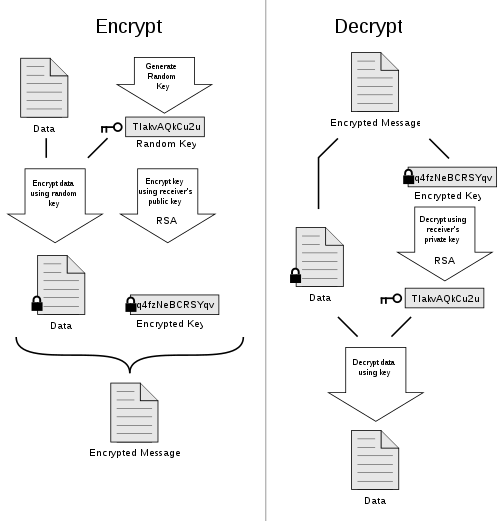
\includegraphics[width=10cm]{images/PGP_101.png}
\centering
\caption{Le fonctionnement global de PGP}
\label{fig:PGP_101}
\end{figure}

\noindent Ce fonctionnement hybride est défendu à cause de la lenteur et la non-praticité d’un chiffrement asymétrique sur un certain nombre de données. Ainsi en chiffrant uniquement la clé symétrique qui a servi à chiffrer le tout l’on peut déchiffrer bien plus rapidement et simplement le message (typiquement avec un chiffrement symétrique tel qu’AES qui a le droit à des instructions dédiées dans certains processeurs). Contrairement à des chiffrements asymétriques qui sont plus contraignants. Et l'on n'utilise pas directement le chiffrement symétrique car il a besoin d'un secret partagé dès le début de la communication.
PGP utilise un système de clés… PGP est aussi critiqué pour son manque de "Forward Secrecy"...
\paragraph*{Propriétés cryptographiques.}
Le problème qui est souvent reproché à PGP c'est qu'il n'implémentes pas de \textit{Forward Secrecy}. La \textit{Forward Secrecy} permet d'affirmer que si l'on a une brèche à un instant \textit{T}, et qu'un attaquant récupère cette clé, il ne pourra pas déchiffrer les anciens messages.
De plus, la gestion des clés PGP est très problématique, en effet lors de mes tests il était difficile de connecter un serveur de clés p. ex. Ou de recevoir une clé d'un correspondant pour la sauvegarder. Et même en la recevant, comment savoir si cette clé n'a pas été modifiée via un \textit{MITM} p.ex. ? -> utiliser un autre canal pour vérifier l'empreinte.
\paragraph*{Web of Trust.}
Comment faire confiance a une clé -> surtout pour email -> Comment initialiser une confiance ?
\paragraph*{Autocrypt.}
Autocrypt est une manière d'échanger des clés entres emails, ces échanges ne sont pas considérés sécurisé par la communauté (Wikipedia -> à creuser). C'est une façon de s'échanger des clés de manière automatisée mais pas forcément sécurisée (utilise les mails).
\paragraph*{Utilisation.}
Pour mes tests j’ai fait en sorte de trouver l’utilisation la plus simple possible pour voir si un utilisateur lambda pouvait arriver à mettre en place ce genre de sécurité. Il s’est avéré que cela était assez simple au départ, mais dès lors que l'on veut envoyer un mail chiffré à un correspondant cela se complique un peu. J’ai juste eu à installer un Add-On sur mon logiciel de messagerie (Thunderbird dans mon cas) qui s’appelle Enigmail. Ensuite Enigmail a générer mes clés PGP (de manière totallement opaque -> à creuser). Puis j’ai écrit un mail, en appuyant sur un petit cadenas mon mail partait chiffré et signé (uniquement si on a la clé du correspondant). Bien, cependant c’est très opaque et on ne sait pas ce qu'Enigmail et Autocrypt font réellement derrière les décors. L’utilisateur doit encore choisir s’il veut chiffrer ses mails ou non par contre il faut que le destinataire utilise PGP et que l’on ait sa clé publique. 
J’ai donc expérimenté à plus bas niveau ce qu’il se passait.
%TODO Aller dans les détails
\subsection{PEP}
\paragraph*{Citation.}
\textit{By default, communications between pep peers always work end-to-end encrypted – no eavesdrop-ping in between shall be possible by design.}
\paragraph*{Utilisation.}
pep assure un chiffrement de bout-en-bout par design, ils n'ont en effet pas de serveurs en soit et chiffre à l'aide d'un \textit{handshake} fait entres les deux personnes via des \textit{trustwords}. Ce sont des mots qu'il faut vérifier entres les deux partis afin d'être sûr que la connexion est bien authentifiée.
\begin{figure}[h!]
    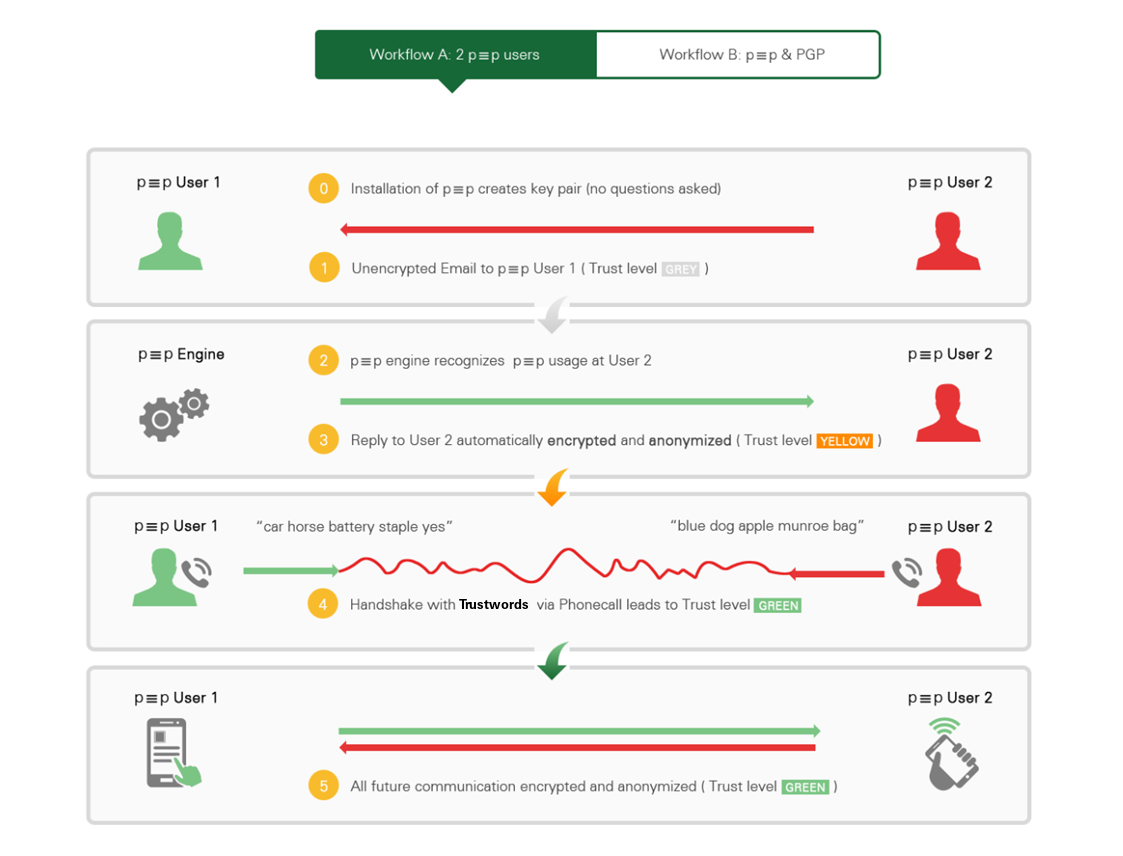
\includegraphics[width=15cm]{images/conceptualpEp.png}
    \centering
    \caption{Le fonctionnement global de pEp}
    \label{fig:PEP_global}
\end{figure}
-> à creuser mais à priori PEP utilise PGP pour le chiffrement des messages.
\subsection{S/MIME}
\label{protocols:SMIME}
\paragraph*{Fonctionnement.}
Basé sur le même principe que PGP principalement, mais avec des certificats pour prouver la légitimité des clés publiques. Pour l'utilisation il faut se créer un certificat, plusieurs classes de confiance existe. 
\paragraph*{Propriétés cryptographiques.}
\paragraph*{Utilisation.}
\section{Implémentations existantes}
\subsection{Protonmail}
\paragraph*{Revendications.}
Protonmail revendique beaucoup de propriétés cryptographiques, tel que le zero-access encryption. Et l’end-to-end chiffrement + zero-knowledge pour les messages sécurisés, même avec leur fonctionnalité de (Chiffrement vers l'extérieur) utilisant AES256-GCM. 
Pour l'authentification Protonmail utilise une manière fortement sécurisée (SRP) pour ne pas avoir d'informations direct sur le mot de passe de l'utilisateur.
\paragraph*{Fonctionnement.}
Protonmail a plusieurs modes de fonctionnement dépendant du destinataire final. En effet de Protonmail à Protonmail les mails sont chiffrés à l'aide de PGP automatiquement. L'on peut utiliser Protonmail pour utiliser PGP si l'on a la clé de notre destinataire par exemple. Et l'on peut écrire un mail chiffré à quelqu'un qui n'utilise pas PGP grâce à une fonctionnalité de chiffrement vers l'extérieur.
Cette fonctionnalité enverra une URL au destinataire qui, en la consultant, pourra déchiffrer le mail en utilisant un mot de passe communiqué de manière sécurisées entres les deux partis auparavant.
\paragraph*{Open Source.}
Tout leur code est open-source afin d'avoir une validation externe, de plus ils ont un programme de Bug Bounty pour les chercheurs.
\subsection{Tutanota}
\paragraph*{Fonctionnement.}
Tout ce que j'ai vu pour le moment c'est que Tutanota utilise AES128-CBC ? Mais dans PGP ou ailleurs ?
%\subsection{Bitmessage}
\section{Attaque existantes}
\subsection{Défauts webmail}
Selon un chercheur~\cite{DBLP:journals/iacr/Kobeissi18a} l'infrastructure de Protonmail aurait des failles via son webmail. Mais son papier est en fait plus général et parle des webmails en règle général.
Il part du principe que les serveurs de Protonmail ne sont pas des serveurs à faire confiance, pour ainsi prouver le zero-knowledge de Protonmail. Par contre, le fait qu'il ne peuvent pas être mis en confiance est un problème selon lui, car c'est ces serveurs qui vont délivrer le code d'OpenPGP afin de faire le chiffrement. 
Cela indique que si Protonmail était corrompu le fait d'avoir le code délivré par Protonmail pourrait avoir des effets néfastes. Comme p.ex l'extraction de la clé privée PGP. La conclusion est que dès le moment où vous avez utilisé une fois le webmail de protonmail la clé PGP est corrompue.
\subsection{EFAIL}
\label{attacks:EFAIL}
Malgré ces sécurités qui pourraient être mises en place à l’heure actuelle, une attaque nommée EFAIL~\cite{DBLP:conf/uss/PoddebniakD0ISF18} a été faite en 2018 et est toujours possible aujourd’hui(à vérifier / tester). En effet cette attaque a seulement été mitigée en évitant d’afficher les contenus HTML et les images dans boites mails de base. Car le problème vient de là principalement, des problèmes sont liés aussi aux modes de chiffrement utilisé (typiquement CBC et CFB) grâce à des "gadgets".
Cette attaque permet en fait d'injecter une image dans l'HTML du message (typiquement dans les headers du mail), puis faire en sorte de récupérer le contenu du message déchiffrer dans un paramètre de l'URL.

\section{Signal}
L'analyse s'est faite aussi pour la messagerie instantanée à cause de sa ressemblance avec la messagerie électronique. 
%Cela m'a finalement permis de me rendre compte que ce n'était pas des protocoles idéaux.
%TODO compléter l'analyse sur Signal
\subsection{Fonctionnement}
%TODO commenter la figure
\begin{figure}[h!]
	\centering
	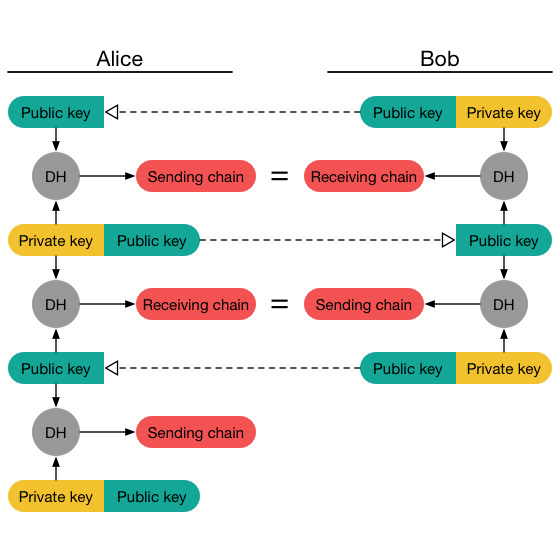
\includegraphics[width=8cm]{images/signalFonctionnement.png}
	\caption{Schéma fonctionnement de Signal\cite{doubleratchet}}
	\label{fig:signal}
\end{figure}
\subsection{Problèmes d'intégrations}
Le problème avec le protocole Signal quant à mes besoins niveaux mails est la \textit{forward secrecy} qui est très fort. En effet comme vu dans le chapitre précédent il utilise une clé par message grâce au \textit{Double Ratchet}. Cependant ce fonctionnement comporte un gros problème en rapport aux mails, en effet si l'on veut pouvoir récupérer les anciens mails reçus/envoyés cela devient vraiment compliqué. En effet, la \textit{forward secrecy} est une propriété utile dans un système de mail, mais faut pouvoir aussi récupérer les messages facilement si l'on connait la clé privée.
\section{Compromis}
Pour passer à l'implémentation concrète d'un nouveau protocole il faut faire des compromis et aller chercher dans des primitives moins connues.\\
Je suis tout de même rester sur un système de clés publiques comme PGP le fait. Cependant cette primitive a une identité propre à chaque clé publique.\\
De plus pour avoir une \textit{forward secrecy} l'on peut ajouter une notion de temps ou de token à l'ID pour chaque batch de messages.
\subsection{Résultats des recherches}
Comme mentionné avant les recherches ont beaucoup été orientées sur le protocole Signal qui a une très bonne forward secrecy, résilience et break-in recovery. Cependant le problème avec l'utilisation des mails c'est d'avoir envie de consulter tout ces mails depuis n'importe quel appareil. Ce n'est malheureusement pas le cas avec Signal à moins de conserver une \textit{root key} quelque part qui ferait s'effondrer les caractéristiques principales du protocole.\\
%TODO : Refaire ce paragraphe
S/MIME est la solution prédominante pour s'envoyer des mails chiffrés cependant il est compliqué de l'utiliser. Il et en effet difficile d'obtenir un certificat pour envoyer des mails et d'échanger avec une autre personne ayant S/MIME.\\
En faisant quelques essais PGP de mon côté je me suis heurté à beaucoup de difficultés et de problèmes avec les clés PGP, notamment pour se les échanger mais pour envoyer ensuite ce n'est pas si complexe, le problème étant de bien voir les primitives utilisées pour chiffrer/signer nore email.
\section{Primitives}
\subsection{Primitives analysées}
%TODO : Expliquer les différentes primitives
- Certificateless PKC~\cite{DBLP:conf/asiacrypt/Al-RiyamiP03}\\
- HIBE - Hierarchised Based encryption\\
- Identity based encryption
%TODO à compléter
\subsection{Primitive choisie}
- Certificateless PKC~\cite{DBLP:conf/asiacrypt/Al-RiyamiP03}\\
Tout d'abord le HIBE aurait été compliqué à mettre en place aussi à cause de sa forte forward secrecy, la hiérarchie doit de plus être commune sur tout les appareils, ce qui prendrait probablement du temps à un nouvel arrivage d'appareil pour un compte donné.
J'ai choisi cette primitive au final car elle proposait des propriétés très intéressantes pour ma manière d'implémenter dans les mails cela. En effet, similaire à de l'identity based avec un ID pour désigner une clé publique. Le problème avec l'identity based encryption c'est le fait que le serveur central génère la clé publique et la clé secrète de l'utilisateur, cela amène ce qu'on appelle le \textit{key escrow} problème. C'est le fait qu'une entité connaisse à elle seule toutes les clés. Ce problème est résolu dans le certificateless en introduisant des \textit{Partial Private Keys} permettant d'avoir une clé secrète partiellement générée par le serveur et par l'utilisateur.
\section{Recherches sur la primitive}
\label{sec:primitiveSearch}
Dans cette section je vais introduire les détails techniques et les principes mathématiques utilisés. De plus, le choix de schéma parmi tous ceux analysés est détaillé ici.
\subsection{Principes mathématiques}
Les variantes de \textit{Certificateless Cryptography} choisies utilisent un concept appelé les \textit{pairings} ou \textit{bilinear map groups}.
Des groupes tels que $\mathbb{G}_1, \mathbb{G}_2, \mathbb{G}_T$ d'un ordre premier \textit{p} pour lesquels il existe un mapping $e : \mathbb{G}_1 \times \mathbb{G}_2 \rightarrow \mathbb{G}_T$ avec les propriétés suivantes :\\
1. Bilinéarité : $e(g^a, h^b) = e(g, h)^{ab}$ pour tout $(g,h) \in \mathbb{G}_1 \times \mathbb{G}_2$ et $a,b \in \mathbb{Z}$;\\
2. Pas de dégénérescence : $e(g,h) \neq 1_{\mathbb{G}_T} $ tant que $g,h \neq 1_{\mathbb{G}_{1,2}}$;
%TODO : Détails mathématiques
\subsection{Schémas Certificateless de Chiffrement}
Pour choisir parmi les nombreux schémas existants en certificateless pour le chiffrement j'ai établi un tableau comparatif des différentes manières de faire, inspiré de~\cite{bookIntroCertificateless}. En suivant ce tableau je me suis rendu compte que la construction de Dent-Libert-Paterson~\cite{DBLP:conf/pkc/DentLP08} était probablement la plus adaptée en vue des propriétés qu'elle présentait. Le tableau se trouve en annexe \ref{ch:fichiers}.
%TODO Expliquer les propriétés et les modèle générique et concret ici
\subsection{À savoir}
Il y a plusieurs choses à savoir avant l'analyse de ces schémas, je vais donc faire une intro en présentant ce qu'il faut savoir sur les propriétés dont je parle ensuite et les différents \textit{Modèles} présents dans la littérature.\\

\subsection{Détails techniques}
Les détails techniques sur le chiffrement avec la \textit{Certificateless Cryptography}.
Le chiffrement se base sur le problème difficile \textit{The Decision 3-Party Diffie-Hellman Problem} (3-DDH). \\C'est de décider si $T =g^{abc} ayant (g^a, g^b, g^c, T) \in \mathbb{G}_4$.\\
Pour expliquer les détails techniques je vais ici montrer les calculs faits dans le schéma choisi~\cite{DBLP:conf/pkc/DentLP08} et les expliquer, cependant dans le schéma il est noté les calculs avec $\mathbb{G} \times \mathbb{G} \rightarrow \mathbb{G}_T$ mais il est mentionné que c'est facilement adaptable pour $\mathbb{G}_1 \times \mathbb{G}_2 \rightarrow \mathbb{G}_T$ ce que j'ai fait. De plus, la conversion vers un groupe additif (travaillant sur les courbes elliptiques) est faite afin que les calculs ici puissent être lus avec mon implémentation :\\
%TODO : mentionner que le prof a aidé / tout fait ?
\textbf{Setup($1^k, n$) :} Avec $\mathbb{G}_1, \mathbb{G}_2, \mathbb{G}_T$ avec un ordre $p > 2^k$. $g$ est un générateur de $\mathbb{G}_1$. Ensuite  $g_1 = g * \gamma$ pour un $\gamma \leftarrow  \mathbb{Z}_p^*$ aléatoire. Puis $g_2 \leftarrow \mathbb{G}_2$. Deux vecteurs (U,V) seront tirés aléatoirement dans $\mathbb{G}_2^{n+1}$ en tant que fonctions de hash notés :
\[F_u(ID) = u' \sum_{i=1}^{n} u_j^{i_j}\quad\mathrm{and}\quad F_v(w) = v' \sum_{i=1}^{n} v_j^{w_j}\]
L'on va aussi prendre une fonction de hash résistante aux collisions : $H : \{0,1\}^* \rightarrow \{0,1\}^n$. Au final notre $mpk$ (master public key) est :
\[mpk \leftarrow (g, g_1, g_2, U, V)\]
Et le $msk$ (master seret key) est $msk \leftarrow g_2*\gamma$.\\
\textbf{Extract($mpk, \gamma, ID$) :} On prend $r \leftarrow \mathbb{Z}_p^*$ puis on retourne $d_{ID} \leftarrow (d_1, d_2) = (g_2*\gamma + F_u(ID)*r, g*r)$\\
\textbf{SetSec($mpk$) :} Retourne un secret aléatoirement choisi $x_{ID} \leftarrow \mathbb{Z}_p^*$.\\
\textbf{SetPub($x_{ID}, mpk$) :} Retourne $pk_{ID} \leftarrow (X,Y) = (g*x_{ID}, g_1*x_{ID})$.\\
\textbf{SetPriv($x_{ID}, d_{ID}, mpk$) :} On choisit $r' \leftarrow \mathbb{Z}_p^*$ puis on reprends $(d_1, d_2) \leftarrow d_{ID}$ et l'on va prendre en secret key : 
%TODO : Revoir si assez complet :
\[sk_{ID} \leftarrow (s_1, s_2) = (d_1*x_{ID} + F_u(ID)*r', d_2*x_{ID} + g*r')\]
Avec $sk_{ID}$ étant la clé secréte de l'utilisateur, donnée par l'Extract (notre Partial Private Key) et la valeur secrète de SetSec.\\
\textbf{Encrypt($m, pk_{ID}, ID, mpk$) :} Pour chiffrer $m \in \mathbb{G}_T$, l'on va reprendre $(X,Y) \leftarrow pk_{ID}$. Pour chiffrer ce message on va tiré aléatoirement $s \leftarrow \mathbb{Z}_p^*$ pui calculer : 
\[C = (C_0, C_1, C_2, C_3) \leftarrow (m + e(Y, g_2)*s, g*s,F_u(ID)*s, F_v(w)*s )\]
Où $w \leftarrow H(C_0,C_1, C_2, ID, pk_{ID})$.\\
\textbf{Decrypt($C, sk_{ID}, mpk$) :} L'on peut reprendre $(C_0,C_1,C_2,C_3) \leftarrow C$ et la clé privée $(s_1, s_2) \leftarrow sk_{ID}$. Afin d'accélerer le déchiffrement le calcul suivant peut être fait en tirant une valeur aléatoire $\alpha \leftarrow \mathbb{Z}_p^*$ :
\[m = C_0 + \frac{e(s_2 + \alpha*g, C_2 )*e(\alpha*g, C_3)}{e(C_1, s_1 + F_u(ID)*\alpha + F_v(w)*\alpha)}\]
Qui donnera $m$ le texte en clair si le chiffré était bien formaté ou un élément aléatoire dans $G_T$.
\subsection{Schémas Certificateless de Signature}
%TODO : Expliquer Malicious KGC et mettre tableaux
Pour choisir parmi les nombreux schémas certificateless pour la signature j'ai établi un tableau comparatif des différentes manières de faire inspiré de~\cite{bookIntroCertificateless}. En analysant les différentes possibilités dans ce tableau il y a peu de solutions se dégage, en effet l'on peut voir que beaucoup de schémas de signature sont cassés, mon choix s'est porté au final sur la construction de Zhang et Zhang~\cite{DBLP:conf/acns/ZhangWXF06} pour des signatures robustes en Certificateless. J'ai pris cette construction car elle est résistante au Malicious KGC (si le KGC a été setup avec des paramètres vulnérables) datant de 2006 et n'a pas été cassée depuis. Le tableau se trouve en annexe \ref{ch:fichiers}.
\subsection{Détails techniques}
Les détails techniques sur la signature avec la \textit{Certificateless Cryptography}.
La signature se base sur le problème difficile \textit{The ComputationalDiffie-Hellman Problem} (CDH). \\Ayant $P, aP, bP$ où $a,b$ aléatoires $\in \mathbb{Z}_q^*$ il n'est pas possible de trouver $abP$.\\
Pour expliquer les détails techniques je vais ici montrer les calculs faits dans le schéma choisi~\cite{DBLP:conf/acns/ZhangWXF06} et les expliquer. Cependant dans le papier original le groupe bilinéaire de couplage choisi est de forme $\mathbb{G}_1 \times \mathbb{G}_2 \rightarrow \mathbb{G}_T$ avec un \textit{pairing} $e(g,h)$ avec $g \in \mathbb{G}_1, h \in \mathbb{G}_2$ alors que le papier annonce une construction tel que $\mathbb{G} \times \mathbb{G} \rightarrow \mathbb{G}_T$.\\
\textbf{Setup($1^k $) :} Tout d'abord l'on va prendre les groupes d'ordre $q$ énoncés auparavant. Puis on choisit un générateur $P \in \mathbb{G}_1$. La \textit{master secret key} va être choisie aléatoirement $s \in \mathbb{Z}_q^*$. Puis la clé publique calculée : $P_{pub} = sP$. Finalement, trois fonctions de hash distinctes $H_1, H_2, H_3$ vont être choisies, chacune d'elle \textit{mappant} de $\{0,1\}^*$ à $\mathbb{G}_2$. Pour cela j'ai choisi de faire du \textit{Hash Domain Separation} comme expliqué dans le Chapitre \ref{ch:impl}. L'on définit les $\mathbf{params} = (\mathbb{G}_1,\mathbb{G}_2,\mathbb{G}_T,e,q,P,P_{pub},H_1,H_2,H_3)$\\
\textbf{Partial-Private-Key-Extract($params, s, ID_A$) :} Pour avoir la \textit{Partial Private Key} ($D_A$) de l'user $A$ avec l'identité $ID_A$. Calculer $Q_A = H_1(ID_A)$. Alors $D_A = sQ_A$.\\
%TODO : Compléter
\textbf{Set-Secret-Value :} La valeur secrète $x \in \mathbb{Z}_q^*$ est tirée aléatoirement.\\
\textbf{Set-Public-Key($params, x$) :}  La clé publique $PK_A$ de l'utilisateur $A$ est $PK_A = xP$.\\
\textbf{Set-Private-Key($params, D_A, x$) :} La clé privé $SK_A$ de l'utilisateur $A$ est calculée comme ceci $SK_A = (D_A, x)$.\\
\textbf{CL-Sign($params, m, ID_A, SK_A$) :} Tout d'abord $r \in \mathbb{Z}_q^*$ est tiré aléatoirement puis on calcules les 2 composantes de la signature :
\[ U = rP\]
\[V = D_A + rH_2(m, ID_A, PK_A,U) + xH_3(m, ID_A, PK_A)\]
Ainsi ces composantes forment la signature $\sigma = (U,V )$.\\
\textbf{CL-Verify($params, PK_A,  m, ID_A, \sigma$) :} Tout d'abord l'on va calculer $Q_A = H_1(ID_A)$ puis effectuer ce calcul afin de vérifier la signature :
\[e(V,P) == e(P_{pub}, Q_A)*e(U, H_2(m, ID_A, PK_A,U))*e(PK_A, H_3(m, ID_A, PK_A)) \]
\section{État de l'art}
Dans cette section je vais analyser et comparer les différentes solutions trouvées utilisant la \textit{Certificateless Cryptography} dans une implémentation concrète pour sécuriser des envois d'emails. J'ai trié les articles suivants par date de publication afin de voir comment les suivants ont repris les technologies etc.
\subsection{Email Encryption System Using Certificateless Public Key Encryption Scheme}
Analyse de l'article~\cite{DBLP:conf/itcs2/ErYTG12}.
\paragraph*{Description.} Cet article présente une façon de faire pour chiffrer les mails à l'aide de \textit{Certificateless Cryptography}. Il va d'abord comparer 6 schémas pour choisir celui à utiliser par rapport à ses propriétés. Ensuite il va comparer les différents algorithmes au niveau du temps avec une implémentation simple en J2SE. 
\paragraph*{Détails techniques.} Les détails techniques ne sont pas très fourni dans cet article, en effet, il est mentionné uniquement le choix du schéma (Whang-Huang-Yang). Puis une comparaison des temps entre les différent algorithmes de la primitive. Finalement ils présentent la différence de temps entre le chiffrement du message via le certificateless et via une clé AES qui est chiffrée avec le certificateless.
%TODO: Expliquer type générique et outsider attacks
\paragraph*{Conclusion.} Ce papier nous conforte dans l'idée de l'utilisation d'AES pour la rapidité du chiffrement qui va avec cette primitive. Cependant, ils n'expliquent pas comment la clé AES est prise et chiffrée réellement. Une implémentation existe en J2SE mais je ne l'ai pas trouvée. Le schéma choisi l'a été pour son avantage de ne pas utiliser les \textit{pairings} et est donc plus rapide. Puis parmi les autres schémas qui n'utilisent pas les \textit{pairings} à ce moment là, un est de type générique et l'autre est vulnérable aux \textit{outsider attacks}.
\subsection{An End-To-End Secure Mail System Based on Certificateless Cryptography in the Standard Model}
Analyse de l'article\footnote{\url{https://www.ijcsi.org/papers/IJCSI-10-2-3-264-271.pdf}}~.
\paragraph*{Description.} Cet article présente une façon de chiffrer et signer dans un systéme de mail avec le schéma original de \textit{Certificateless Cryptography} à savoir le schéma d'Al-Riyami et Paterson~\cite{DBLP:conf/asiacrypt/Al-RiyamiP03}. Un article complet définissant bien le contexte de mails et formalisant pour la première fois un moyen de chiffrer et signer des mails avec de la \textit{Certificateless Cryptography}. Cela en expliquant dans les détails comment ils feraient, sans implémentations citées de ce schéma.
%TODO A voir, j'ai l'impression qu'il y a une erreur dans le papier pour le déchiffrement de t*
\paragraph*{Détails techniques.} Les détails techniques intéressant dans ce papier est la manière d'encapsuler la clé de chiffrement du message. Sinon le reste s'appuie sur le schéma d'Al-Riyami et Paterson.
Pour établir une clé de chiffrement symmétrique afin de chiffrer le mail l'n va tout d'abord tirer une valeur aléatoire $t \in \mathbb{Z}_p$ puis la chiffrer avec CL-PKC en utilisant la clé publique du destinataire $t* = Enc_{P_B}$. Ce $t^*$ sera envoyé avec l' email. Pour en tirer une clé symmétrique on va établire : $K_{AB} = tx_AP_B$ à l'aide de la clé privée de la source et la clé publique du destinataire et enfin la valeur aléatoire tirée auparavant. Puis l'on va calculer la clé symmétrique $K = H_2(Q_A||Q_B||K_{AB})$.
\paragraph*{Conclusion.} Ce papier est assez complet concernant la partie fonctionnement des mails en globalité et offres une bonne idée pour la construction d'une clé symmétrique par mail envoyé. Cependant la mise en place de la clé symmétrique et la preuve de son fonctionnement n'est pas très explicitée. D'ailleurs il y a selon moi une erreur dans le papier original pour la logique de déchiffrement de $t^*$ et de la récupération de la clé symmétrique. De plus, le systéme de signature d'Al-Riyami et Paterson a été cassé par~\cite{DBLP:conf/cans/HuangSMZ05}.
\subsection{Practical Implementation of a Secure Email System Using Certificateless Cryptography and Domain Name System}
Analyse de l'article~\cite{DBLP:journals/ijnsec/BalakrishnanR16}.
\paragraph*{Description.} Ce papier traite le problème de la même façon que le précédent mais essaies d'aller plus loin dans les détails d'un implémentation à plus grande échele (utilisation DNS). Il reprend le même schéma et les mêmes principes pour la création de la clé symmétrique de chiffrement. Le même schéma de signature est présent aussi, qui est cassé rappelons-le. Le but serait d'avoir une entrée DNS similaire au DKIM déjà utilisé pour les emails afin d'informer les utilisateurs quelle adresse donne es clés publiques du domaine en question.
\paragraph*{Détails techniques.} Beaucoup de détails concernant les domain policies qui pourraient être appliqués aux domaines pour la distribution des clés publiques. Proposition d'utiliser les headers d'emails pour transmettre la signature de l'email et informer le destinataire si l'email est chiffré ou non et de transmettre les IDS utilisés et le TImestamp utilisé. En effet, l'introduction d'un timestamp est proposé ici pour avoir un temps d'expiration au mail. Les DOmain Policies sont là pour informer les utilisateurs si les emails de ce domaines doivent être signés/chiffrés ou non.
\paragraph*{Conclusion.} Une implémentation est citée utilisant la librairie MIRACL et en utilisant le C++ comme langage de programmation. L'implémentation est citée comme extension \textit{Thunderbird} en C++ / Javascript. Mais il n'y a pas de réel guide pour implémenter cela au monde réel avec des exemples de configuration DNS et autres. Pas vraiment d'explications sur l'utilisation d'une multitude de KGC ou un seul central, comment les synchroniser et autres... Par contre beaucoup d'explications sur comment pourrait fonctionner une entrée DNS afin d'informer aux utilisateurs où aller pour récupérer les clés publiques des utilisateurs du domaine en question et des policies qui pourraient s'appliquer à ce domaine.
\subsection{PriviPK : Certificate-less and secure email communication}
Analyse de l'article~\cite{DBLP:journals/compsec/AlSabahTLSD17}.
\paragraph*{Description.} Cet article propose une implémentation très concréte utilisant CL-PKC pour communiquer de manière sécurisée dans la messagerie éléctronique. Il attaque beaucoup d'aspects que les autres papiers n'ont pas mentionnés comme la \textit{key transparency}. Le papier insiste sur la transparence du protocole pour l'utilisateur afin qu'il n'ait pas d'opérations fastidieuses à faire (comme c'est le cas dans PGP et S/MIME par exemple). Ce papier s'appuie sur un systéme de \textit{key agreement} proposé dans la littérature de la cryptographie basée sur l'identité.
\paragraph*{Détails techniques.} CONIKS serveur, authentification via les clients mails déjà existants (gmail et yahoo), mise en place d'un systéme de key agreement id-based repensée pour le certificateless.
\paragraph*{Conclusion.} Ce papier est assez intéressant et c'est la seule véritable implémentation que j'ai trouvée, il y a un repo sur github. Cependant il s'appuie sur du \textit{key agreement}. Comme le prochain systéme d'ailleurs. Par aileurs, il insiste sur la transparence et sur l'utilisation des authentifications déjà présentes sur les clients emails.
\subsection{A certificateless one-way group key agreement protocol for end-to-end email encryption}
Analyse de l'article~\cite{DBLP:conf/prdc/YehSDSSW18}.
\paragraph*{Description.} Dans cet article les auteurs présentent un moyen d'avoir une clé partagée entre n-partis et avec un seul message, ce qui permet dans un systéme de mail d'avoir qu'à envoyer un mail avec les informations nécessaires pour recomposer la clé partagée. Cette clé partagée est utilisée afin de chiffrer le mail et de l'envoyer ensuite avec les informations nécessaires à la création de la clé partagée. De plus, le systéme est n-parti, cela veut dire que l'on peut envoyer le mail à n personnes et le chiffrer avec la même clé. On enverra juste pas les mêmes informations de créations de la clé partagée à tous.
\paragraph*{Détails techniques.} Pour ce qui est des détails techniques on peut voir que le principe est de créer une clé partagée à l'aide des différents ID et clés publiques des destinataires. On aura une sous-clé $x_i$ pour chaque utilisateur $i$. L'on va construire un $y_i = x_0 \dots x_{i-1} + x_{i+1} \dots x_n$ pour un utilisateur où l'on additionnera tout les $x$ des utilisateurs sauf de l'utilisateur $i$. Ainsi à la réception du message l'utilisateur pourra recréer la clé partagée en faisant $y_i + x_i = x_0 + \dots + x_n = K$. Ce $K$ sera ensuite utilisé pour chiffrer le mail.
\paragraph*{Conclusion.} Ce systéme est simple et efficace mais ne permets pas la signature des éléments nécessaires à la création de la clé partagée, l'on peut donc envisager des DOS afin qu'un utilisateur ne puisses plus lire ces messages. Cependant c'est une construction intéressante se basant sur un \textit{key-agreement} via le \textit{Certificateless Cryptography} et non pas sur ses possibilités de chiffrement/signature.



